
\documentclass{paper}

\usepackage[a4paper,margin=2cm]{geometry}
\usepackage{multicol}

%%%%%%%%%%%%%%%%%%%%%%%% to make pandoc work

\def\tightlist{} % make \tightlist do nothing https://tex.stackexchange.com/questions/257418/error-tightlist-converting-md-file-into-pdf-using-pandoc/408474
\newcommand{\passthrough}[1]{\lstset{mathescape=false}#1\lstset{mathescape=true}} % from  https://github.com/laboon/ebook/issues/139


%%%%%%%%%%%%%%%%%%%%%%%%

% code handling
 \usepackage{listings}
%\usepackage{minted} % 18jan2022, not working yet
\usepackage{xcolor}
\usepackage[lighttt]{lmodern}
% \usepackage{pretty_verilog}

% so algorithms can work within multicol
\usepackage{float}

% for flowcharts
\usepackage{tikz}

% For figures
\usepackage{graphicx}% more modern
% \usepackage{subfigure}
\usepackage[font=small,labelfont=bf]{caption} % Required for specifying captions to tables and figures
\usepackage[subrefformat=parens]{subcaption} % from https://tex.stackexchange.com/questions/238636/add-caption-to-image-included-with-includegraphics-within-center-environment

% For dates
\usepackage{datetime}

% For citations
% \usepackage{biblatex}
% \addbibresource{main.bib}
\usepackage[
  backend=biber,
  bibencoding=utf8
]{biblatex}
% \addbibresource{content/part_b:_projects/references.bib}

\usepackage[nottoc]{tocbibind} % So the citations appears in the TOC (table of contents)
% for controlling toc indents, from https://tex.stackexchange.com/questions/111478/how-to-add-more-indentation-for-section-in-table-of-contents
\usepackage{tocloft}%,tocloft} titletoc
\setlength{\cftsubsecindent}{0.5cm}
% \setlength{\cftsubsubsecindent}{1cm}
% \dottedcontents{section}[1.5em]{}{1.3em}{.6em}

% For algorithms 
% \usepackage{algorithm}
% \usepackage{algorithmic}
\usepackage[ruled,vlined]{algorithm2e}

% to render URLs with underscores correctly
\usepackage{url}

% to produce hyperlinks in the resulting PDF.
\usepackage{hyperref}
\hypersetup{
    colorlinks=true,	% make the links colored
    % hidelinks=true
}

% to add progress comments feedback 
\usepackage[colorinlistoftodos,prependcaption]{todonotes} %,textsize=tiny
\presetkeys{todonotes}{inline}{}

% for using separate files
% \usepackage{subfiles}% Best loaded last in the preamble

% so paragraphs don't have the starting indent
\setlength{\parindent}{0in}

\title{Some title}
\subtitle{And a small subtitle}
% \author{General Documentation}

\begin{document}
\begin{multicols*}{2}

\maketitle
% \subfile{content/abstract}
% \subfile{content/terminology}
% \subfile{content/progress}
\vfill\null
\columnbreak

\setcounter{tocdepth}{2}
\tableofcontents

\end{multicols*}
% \hrulefill

% \subfile{content/section_a:_plan_overview/plan_overview}

% \subfile{content/section_b:_hardware_overview/hardware_overview}

% verilog language


\part{This is part one}

\hypertarget{heading-one-in-main.md}{%
\section{heading one in /main.md}\label{heading-one-in-main.md}}

Edit made on new os.

\textbf{paragraph} in /main.md

note the things in \textbf{parts} must be \emph{directories} which
contain a main.md. That main.md file may also have a \textbf{parts}
section for including further files, etc.

\begin{figure}
\centering
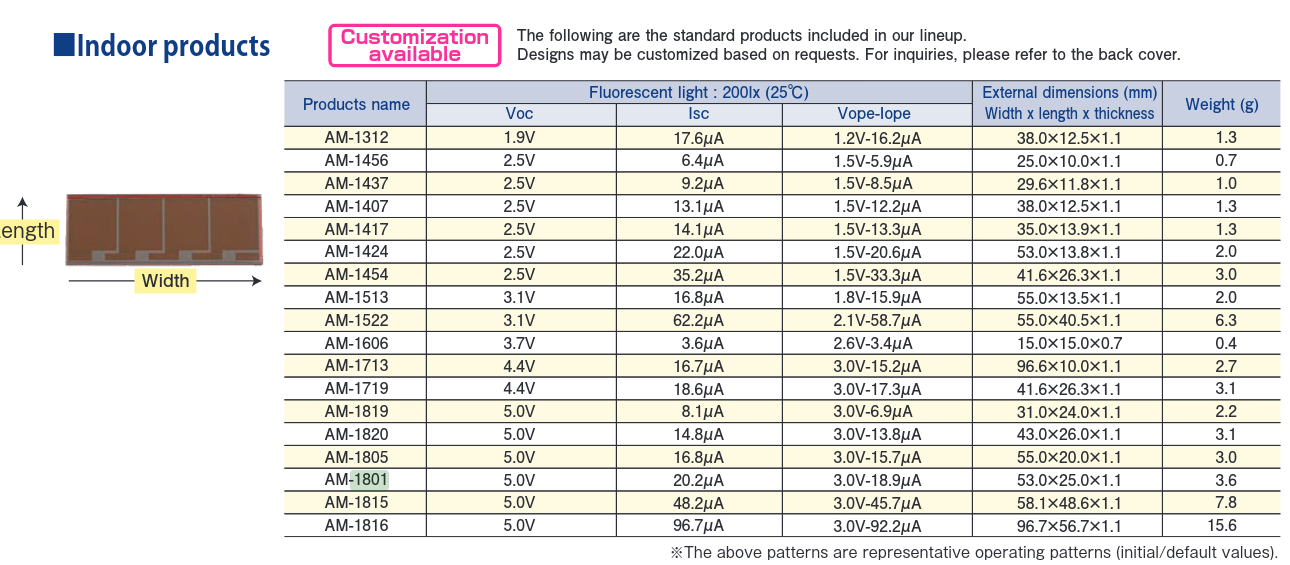
\includegraphics{/home/ubuntu/Documents/Uploads/content/./panasonic_amorton_indoor_list.png}
\caption{alt text}
\end{figure}

\part{This is part two}

\hypertarget{to-do}{%
\section{To do}\label{to-do}}

\begin{itemize}
\tightlist
\item
  Closely match the appearance of my latex documents from a year ago

  \begin{itemize}
  \tightlist
  \item
    same border spacing
  \item
    same structure, e.g.~have an abstract/terminology/progress sections,
    bibliography/appendix etc
  \item
    make top level headings as `parts', e.g.~part 1, part 2,
  \end{itemize}
\end{itemize}

well let's consider this algorithm

\begin{lstlisting}[language=Python]
def mainko(bozo):
    return "hungry"
\end{lstlisting}

as well as this

\begin{lstlisting}[language=C]
int mainko(int bozo){
    return ERROR_UNDEF;
}
\end{lstlisting}

\hypertarget{heading-level-2-in-the-.md}{%
\section{heading level 2 in the .md}\label{heading-level-2-in-the-.md}}

aaa

\hypertarget{heading-level-3-in-the-.md}{%
\subsection{heading level 3 in the
.md}\label{heading-level-3-in-the-.md}}

bbb

todo - make the key:value thing in parts be section parts to filenames,
e.g.~for abstract, progress, etc?

\hypertarget{heading-level-1-should-become-2-in-contenta_outerfoldermain.md}{%
\section{Heading level 1 (should become 2) in
content/a\_outerfolder/main.md}\label{heading-level-1-should-become-2-in-contenta_outerfoldermain.md}}

Content below that heading in the markdown file

\hypertarget{heading-level-1-should-become-2-in-contentb_outerfoldermain.md}{%
\section{Heading level 1 (should become 2) in
content/b\_outerfolder/main.md}\label{heading-level-1-should-become-2-in-contentb_outerfoldermain.md}}

Content below that heading in the markdown file. A nested list test
follows.

\begin{enumerate}
\def\labelenumi{\arabic{enumi}.}
\tightlist
\item
  This is one element
\item
  Another

  \begin{enumerate}
  \def\labelenumii{\arabic{enumii}.}
  \tightlist
  \item
    And a nested element

    \begin{itemize}
    \tightlist
    \item
      with a nested dot
    \item
      another
    \end{itemize}
  \item
    More element
  \end{enumerate}
\item
  Outer end of list
\end{enumerate}

Note that there are two more subfolders here, however they are not
referenced in this markdown file, and hence are not integrated into the
final document.

\hypertarget{heading-level-1-should-become-2-in-contentc_outerfoldermain.md}{%
\section{Heading level 1 (should become 2) in
content/c\_outerfolder/main.md}\label{heading-level-1-should-become-2-in-contentc_outerfoldermain.md}}

ffbc

\hypertarget{hello-from-behe}{%
\subsection{hello from behe}\label{hello-from-behe}}

hohoe

\hypertarget{jfdksllkjfdslkjfds}{%
\subsubsection{jfdksllkjfdslkjfds}\label{jfdksllkjfdslkjfds}}

bo how bew stant

\hypertarget{hullow-from-b_boho}{%
\subsection{hullow from b\_boho}\label{hullow-from-b_boho}}

as a paragraph

\begin{figure}
\centering
\includegraphics{/home/ubuntu/Documents/Uploads/content/c_outerfolder/b_boho/./panasonic_amorton_indoor_list2.png}
\caption{alt text}
\end{figure}

\hypertarget{as-a-second-level-heading}{%
\subsubsection{as a second level
heading}\label{as-a-second-level-heading}}

huahua

another end line\ldots{} helps?
\includegraphics{/home/ubuntu/Documents/Uploads/content/c_outerfolder/./b_boho/panasonic_amorton_indoor_list2.png}

\hypertarget{hellobd}{%
\section{hellobd}\label{hellobd}}

ffbd

\part{another top level heading}

here's a copy-pasted thing of the parts - does it work?

\end{document}